\section{Introduction}
\label{sec:introduction}


\begin{figure}[t]
\centering
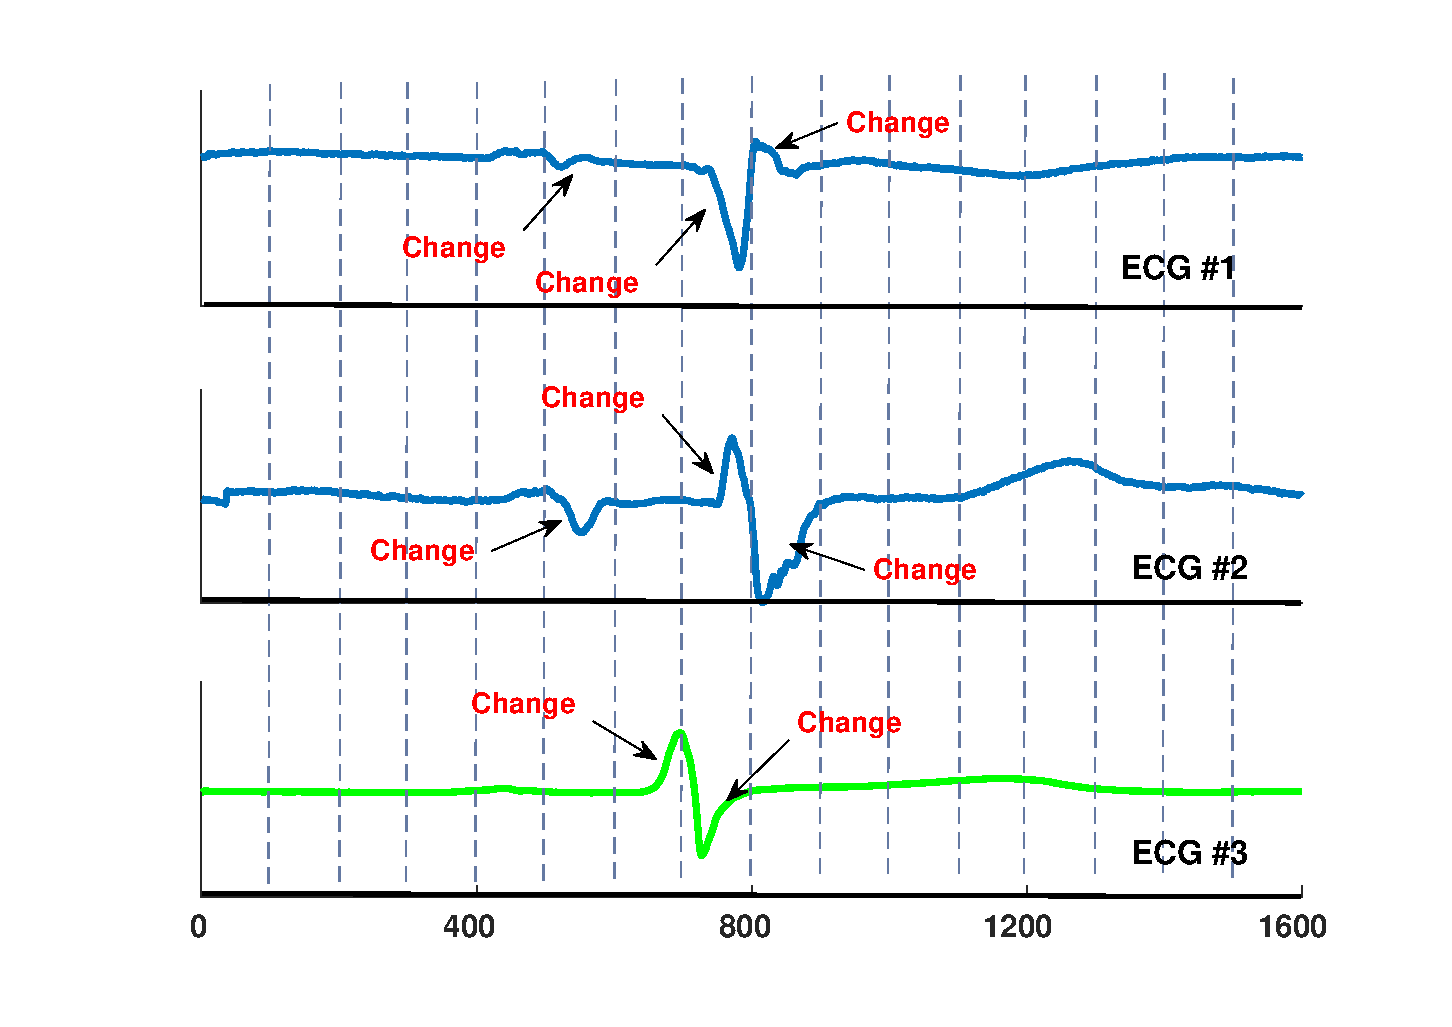
\includegraphics[width=0.45\textwidth]{ECGexp.eps}
\caption{ Three ECG time series with two labels }
\label{fig:ecgexample}
\end{figure}

\begin{figure}[t]
\centering
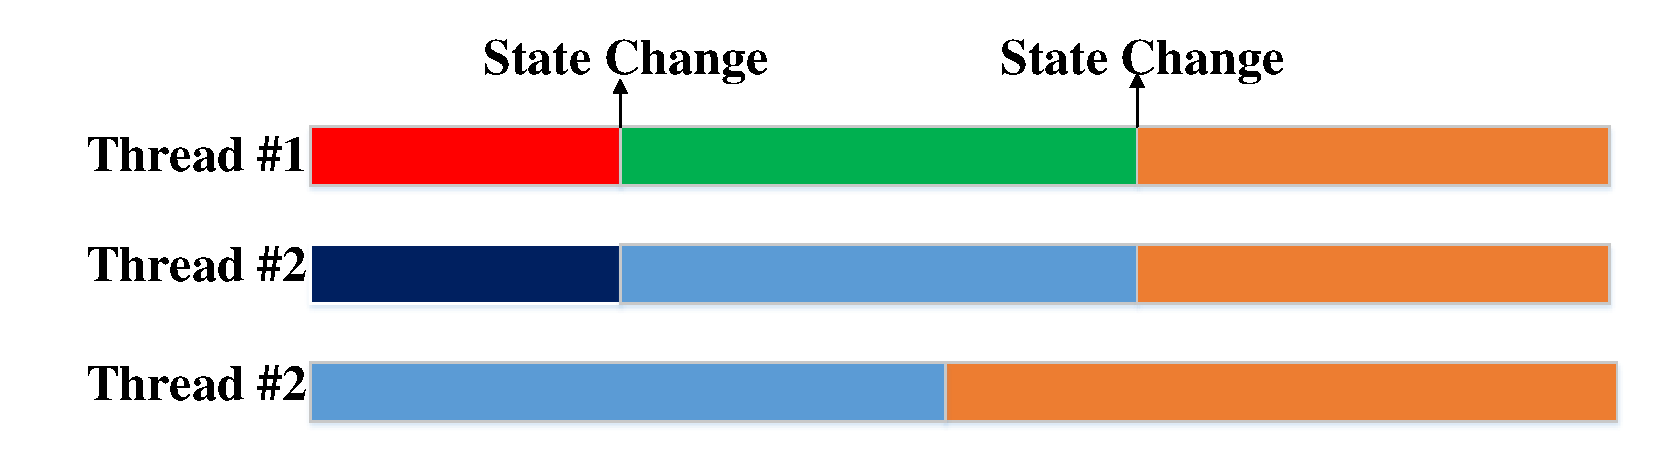
\includegraphics[width=0.45\textwidth]{HPCExample.pdf}
\caption{Three Thread time series}
\label{fig:hpcexample}
\end{figure}

Time series correlation is a major research topic in data mining area. 
Such correlating techniques have been applied to many real-world problems.
For example, some researchers use time series correlation techniques to analysis the signal information for speech processing \cite{rabiner1993fundamentals}.
Image processing researchers also use time series correlation techniques to deal with the image retrieval problems and object detection problems \cite{yang2002detecting, sonka2014image}.
In the system diagnose area\cite{luo2014correlating,sun2014querying}, time series correlation techniques also widely used to mine the system behavior and diagnose system failures. 
Time series correlation techniques can also be used for analyzing bio-sequences (e.g DNA Sequence, etc \cite{mount2001bioinformatics} etc. 

However, in most real-world problems, time series data often have different patterns (e.g. Periodical, Linear, random, etc.).  And the correlation between these heterogeneous time series is also very meaningful.
Despite their importance, there has been little previous work addressing the correlation between two types of heterogeneous time series data. We provide two motivating example as bellow:

\textbf{Analysis of ECG (Electrocardiogram) data}

Electrocardiography \cite{holter1961new} (ECG or EKG*) 
is the process of recording the electrical activity of the heart over a period of time using electrodes placed on a patient's body. 
These electrodes detect the tiny electrical changes on the skin that arise from the heart muscle depolarizing during each heartbeat. 
By analyzing such data, one can find some useful information hidden behind the human body, thus to uncover some miracle of human body \cite{tilley1979essentials}.

Such ECG data can be regarded as time series data. Detect the correlation between each ECG time series can provide useful information for analyzing ECG data. 
After knowing the correlation between different ECG data, one can use such correlation result to find the hidden relationship between each human and diseases \cite{marriott1988practical}.

However, we can see from Fig.\ref{fig:ecgexample} that, ECG time series data correlation are regarded as tiny electrical change at the same time \cite{tilley1979essentials}. And the change has different patterns. As a result, some classical similarity or correlation method can not deal with such problem well, even DTW sometimes also fail to detect such patterns. As a result, a change based correlation is needed.


\textbf{Thread Behavior Mining in High Performance Computer.}
High performance computers (HPC) have become enormously complex. Today, the largest systems consist of more than tens of thousands of nodes. Nodes themselves are equipped with one or more multicore microprocessors\cite{adhianto2010hpctoolkit}. 

As a result, it is increasingly difficult for application developers writing complex scientific programs to attain a significant fraction of peak performance on modern microprocessor-based computer systems. 
So, how to automatically analysis and monitoring the HPC is a major task for HPC researchers \cite{mccurdy2010memphis,tallent2009effective}.

HPCToolkit\footnote{http://hpctoolkit.org/}, introduced by Dr.John Mellor-Crummey, can generate some performance information of each process (or thread if the application is multithreaded.) along the time. So, each process (thread) can be represented as a time series (Depend on which aspect of a thread to be represented, domain knowledge required). The thread change information (e.g. change from one state to another state) can directly reflect some important properties of different threads. 

Fig. \ref{fig:hpcexample} shows an example of three thread time series data. From the figure, we can see that above two thread often change at the same time, so they may have a high correlation between each other. However, using the point to point based similarity method (e.g. DTW, Pearson, etc.), we can not handle such heterogeneity property of different thread time series.

As showed in above examples, most of the existing point to point time series similarity measures (e.g. L1-Distance, L2-Distance \cite{han2011data}, and DTW-Distance \cite{muller2007dynamic}, etc) or correlation measures (e.g. Pearson Correlation \cite{pearson1904mathematical}, Kendall rank correlation \cite{kendall1938new}, and Spearman's rank correlation \cite{pirie1988spearman}, etc.) can not deal with such heterogeneous properties of the time series. 
The reason is: for heterogeneous time series, the correlation information is often associated with the change (During a period of time) of time series, rather than a point-to-point relationship in the traditional correlation analysis techniques. We will introduce the related research of point to point based similarity measure in detail in Section \ref{sec:relatedwork}.

As a result, in order to deal with heterogeneity properties of time series, we proposed a change based correlation coefficient. 
The intuition of this correlation is: 
\textbf{\textit{If two time series often change at the same time, they may have correlation with each other.} }. The mathematical definition of change based correlation is introduced in section \ref{sec:formulation}. 

Our change based correlation method firstly extract the change information of the time series data, and then use the change information to calculate the correlation coefficient between the two time series.
By taking the advantage of this correlation coefficient, we propose to use LSH method to dealing with very large top-k searching problems.

The contribution of this paper is listed as follow:
\begin{enumerate}
\item Motivated by real applications, we investigate the correlation
problem as between heterogeneous time series .
To the best of our knowledge, this is the first attempt
to evaluate the correlation between time series with different patterns.

\item We proposed a correlation coefficient between heterogeneous time series. By taking the advantage of this correlation coefficient, we propose to use LSH method to dealing with very large top-k searching problems.

\item The experiments on Synthetic data sets and Real world data sets show the effectiveness and efficiency of our method.
\end{enumerate}

The rest of the paper is organized as follows: In Section 2, we introduce the problem
statement and formulation. Our approach is proposed in Section 3. The Empirical evaluation is shown in Section 4. In Section 5, we introduce some
related works. Finally, we conclude our work in Section 6.



